\documentclass[10pt,a4paper]{article}
\usepackage[utf8]{inputenc}
\usepackage[francais]{babel}
\usepackage[T1]{fontenc}
\usepackage{amsmath}
\usepackage{amsfonts}
\usepackage{amssymb}
\usepackage{graphicx}
\usepackage{enumitem}
\usepackage{lmodern}
\usepackage{listings}
\usepackage{color}
\usepackage{tikz}

\definecolor{mygreen}{rgb}{0,0.6,0}
\definecolor{mygray}{rgb}{0.5,0.5,0.5}
\definecolor{mymauve}{rgb}{0.58,0,0.82}

\lstset{ %
  backgroundcolor=\color{white},   % choose the background color; you must add \usepackage{color} or \usepackage{xcolor}
  basicstyle=\footnotesize,        % the size of the fonts that are used for the code
  breakatwhitespace=false,         % sets if automatic breaks should only happen at whitespace
  breaklines=true,                 % sets automatic line breaking
  captionpos=b,                    % sets the caption-position to bottom
  commentstyle=\color{mygreen},    % comment style
  deletekeywords={...},            % if you want to delete keywords from the given language
  escapeinside={\%*}{*)},          % if you want to add LaTeX within your code
  extendedchars=true,              % lets you use non-ASCII characters; for 8-bits encodings only, does not work with UTF-8
  frame=single,                    % adds a frame around the code
  keepspaces=true,                 % keeps spaces in text, useful for keeping indentation of code (possibly needs columns=flexible)
  keywordstyle=\color{blue},       % keyword style
  language=Java,                   % the language of the code
  morekeywords={*,...},            % if you want to add more keywords to the set
  numbers=left,                    % where to put the line-numbers; possible values are (none, left, right)
  numbersep=5pt,                   % how far the line-numbers are from the code
  numberstyle=\tiny\color{mygray}, % the style that is used for the line-numbers
  rulecolor=\color{black},         % if not set, the frame-color may be changed on line-breaks within not-black text (e.g. comments (green here))
  showspaces=false,                % show spaces everywhere adding particular underscores; it overrides 'showstringspaces'
  showstringspaces=false,          % underline spaces within strings only
  showtabs=false,                  % show tabs within strings adding particular underscores
  stepnumber=2,                    % the step between two line-numbers. If it's 1, each line will be numbered
  stringstyle=\color{mymauve},     % string literal style
  tabsize=4,                       % sets default tabsize to 2 spaces
  title=\lstname                   % show the filename of files included with \lstinputlisting; also try caption instead of title
}
\usepackage[left=2cm,right=2cm,top=2cm,bottom=2cm]{geometry}


\date{Vendredi 28 Novembre 2014}
\author{Groupe 2.2}
\title{Mission 5 : Rapport Final}
\begin{document}
\maketitle
\section*{Introduction}
Il nous a été demandé de réaliser un programme de compression et de décompression de fichiers. Ce programme devait s'inspirer de l'algorithme de Huffman. Le codage de Huffman faisant appel à une file de priorité, il était nécessaire d'implementer cette file de la manière la plus efficace possible.

\section*{Choix d'implémentation}
Le programme comporte 5 classes, InputBitStream, OutputBitStream, Compress, Decompress, HTree. Les deux premières classes citées, nous ont été fournies. Vous trpuverez ci-dessous une explication pour chacune d'elles.

\subsection*{InputBitStream et OutputBitStream (Question 7)}
De manière générale, des données textuelles sont codées soit en utilisant la norme ASCII, soit la norme UNICODE, qui font toutes deux correspondre un code binaire de 7 ou 16 bits à chaque caractère. L'algorithme d'Huffman va remplacer cette suite de bits de taille fixe par une suite de taille variable en fonction de la fréquence de chaque caractère dans le texte à traiter, et cela de manière optimale (les chaines de bits les plus courtes correspondront aux caractères apparaissant le plus souvent dans le texte et inversément).\\

	Les deux classes InputBitStream et OutputBitStream permettent d'écrire un fichier directement en binaire, donc de contourner l'encodage ASCII ou UNICODE par défaut, et sont de ce fait nécessaire à la réalisation de l'algorithme d'Huffman.\\
	
	Cependant, le fait d'utiliser des correspondances de taille variable entraine que la taille totale peut ne pas etre un multiple de 8 bits (1byte) et donc etre complété par des 0 pour terminer le dernier byte entammé. Pour gérer ce problème, nous avons intégré au header une suite de bits indiquant le nombre de caractères dans le fichier. Lorsque ce nombre de caractères déchiffrés est atteint à la décompression, cela signifie que l'ensemble des données ont été décompressées, et le programme ne tient donc pas compte des bits additionnels.

\subsection*{Compress}
La classe Compress va lire une première fois le fichier source caractère par caractère pour créer une table de fréquence, qui est une hashMap ayant pour clé un caractère et comme valeur une fréquence. Avec les informations de la table de fréquence, nous créons l'arbre de Huffman et un table de traduction, c'est aussi une hashMap ayant pour clé le caractère compressé et pour valeur un string contenant la valeur du caractère compressé. \\
Nous créons un fichier ayant pour entête les informations suivantes :

$| byte (8b) -> 3 si version 1.3$ \\
 $ | short (16b) -> number of characters in dictionary (->n)$\\
 $ | long (64b) -> number of characters in file $\\
$    n*| char (16b) -> character $\\
  $    | int (32b) -> codeword, left-padded with 00..01 $\\
 $ | (variable length, binary) -> compressed data $\\

Ensuite, nous parcourons une seconde fois le fichier sources à l'aide de la table de traduction pour transcrire les différents caractères rencontrés en caractères compressés sur le fichier compressé.

\subsection*{Decompress}

Dans un premier temps, nous lisons les informations contenue dans l'entête du fichier compressé. A partir de ces informations, nous créons une nouvelle table de traduction, ayant comme clé un string représentant la valeur d'un caractère compressé et comme valeur le caractère référencé. Nous parcourons le fichier bit par bit et à chaque nouveau bit, nous cherchons une correspondance entre le buffer de bits et une clé de la table de traduction. Lorsqu'il y a correspondance, nous écrivons la valeur de la table de traduction dans le fichier décompressé et nous vidons de buffer. Nous continuons ainsi de suite jusqu'à la fin du fichier qui est connue car nous connaissons le nombre de caractères présents dans le fichier grâce à l'entête.

\subsection*{HTree}
La classe HTree utilise un SetMap contenant tous les caractères utilisés dans le fichier ainsi que leur fréquence pour créer un arbre de Huffman à l'aide d'une priorityQueue. L'abre de Huffman ainsi créé est ensuite parcouru de manière récussive pour créer un Hashmap contenant les caractères comme clé et comme valeur un string représentant ce caractère compressé.
Nous avons pris la décision d'implémenter complétement la classe HTree et donc de ne pas étendre la classe générique TreeSet. L'avantage de cette approche, c'est que cette classe correspond exactement à ce qu'on attend d'elle. Par contre, l'inconvénient c'est que l'on perd en portabilité.


\section*{Diagramme de classe (Question 8)}
\begin{center}
<<<<<<< Updated upstream
%<<<<<<< HEAD
    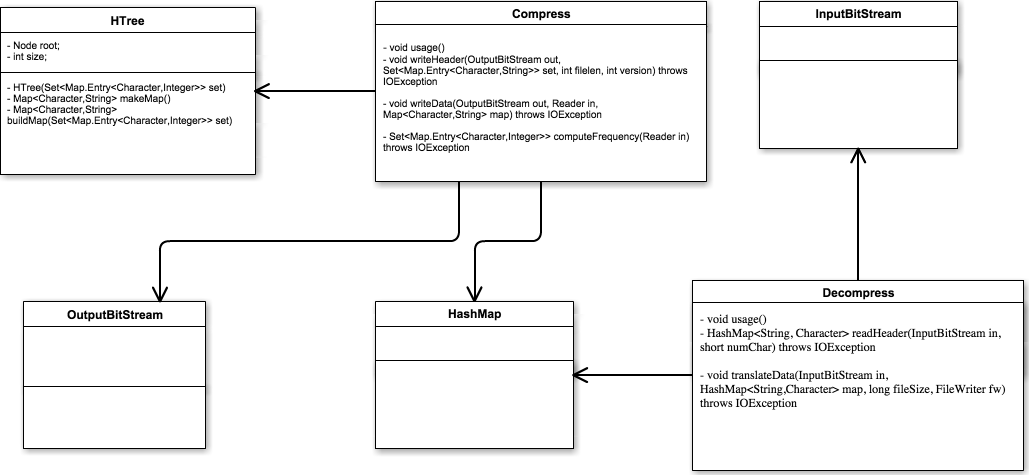
\includegraphics[scale=0.5]{UML.png}
%=======
   % 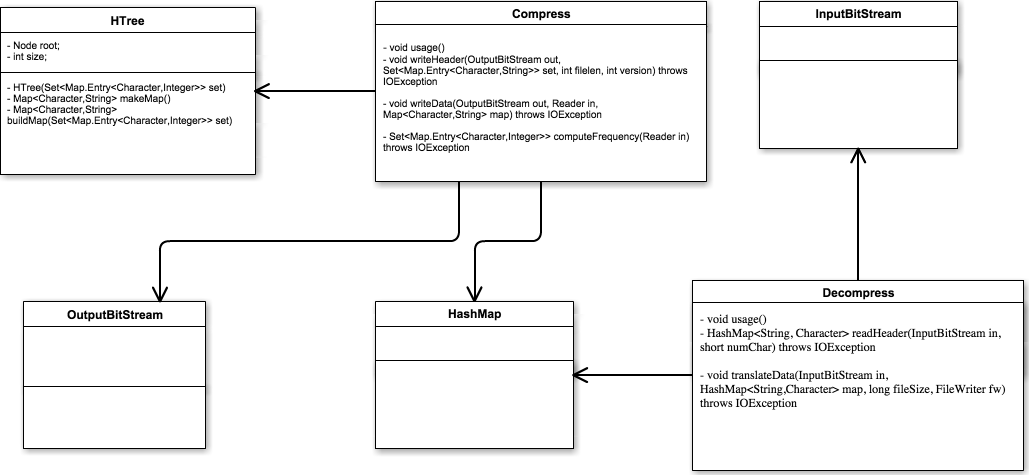
\includegraphics[scale=0.4]{Class_Diagram.png}
%>>>>>>> FETCH_HEAD
=======
    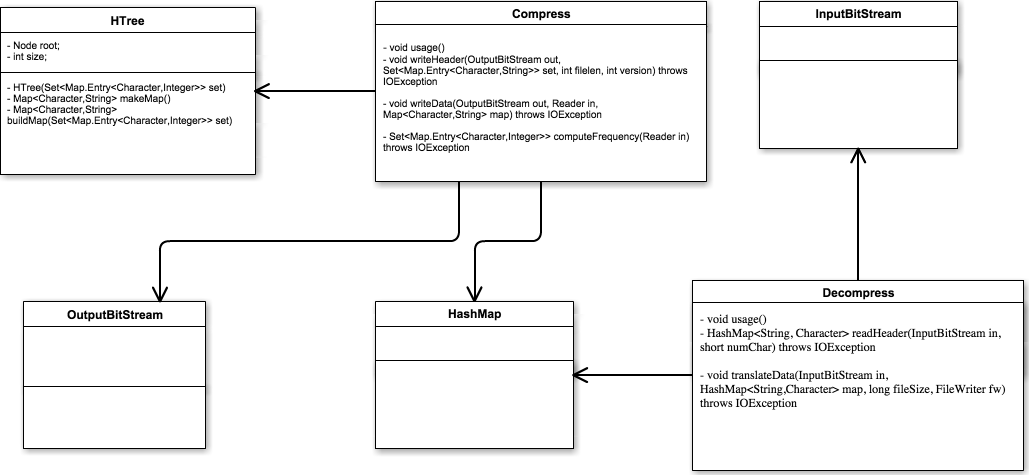
\includegraphics[scale=0.4]{UML.png}
>>>>>>> Stashed changes
\end{center}

\section*{Test (Question 9 et 10)}

Vu que nous avons utilisé l'algorithme de compression par codage de Huffman pour notre code, nous pouvons supposer que notre implémentation est normalement sans perte. Mais qu'est-ce que ça signifie un compression sans perte ? \\ Une compression est sans perte lorsqu'il y a autant d'informations avant et après la compression. Les fichiers compressés et ensuite décompressés doivent être en tout point identique.\\
L'approche que nous utilisons pour compresser les fichiers nous permet d'affirmer que la compression est sans perte. En effet, nous gardons dans l'entête du fichier compressé différentes informations permettant la bonne décompression de ce fichier, dans cette entête se trouve un "dictionnaire" nous permettant de faire correspondre chacun des caractères compressés avec son caractère source. La table de traduction a été construite avec l'ensemble des caractères rencontrées dans le fichier source. \\La méthode la plus fastidieuse de vérifié que notre implémentation de compression et de décompression est sans perte serait de comparer caractère par caractère le fichier source et le fichier décompressé. D'après nous, la manière la plus efficace de tester la validité de cette affirmation est de comparer le nombre de caractères du fichier source et de fichier décompresser.

\section*{Conclusion}
La décomposition des classes dans notre programme, nous a facilité la répartition des taches, l'utilisation de multiple classe permet aussi de pouvoir être plus modulable. Tant au niveau de la repartition du travail, qu'au niveau de l'ajout de nouvelles fonctions pour adapter notre programme.\\ 

\end{document}